\documentclass[a4paper, 11pt]{article}
\usepackage{comment} % enables the use of multi-line comments (\ifx \fi) 
\usepackage{fullpage} % changes the margin
\usepackage{blindtext}
\usepackage{tabularx,colortbl}
%\usepackage{psfig}
%\usepackage{siunitx}
\usepackage[final]{pdfpages}
\usepackage{graphicx}
\usepackage[utf8]{inputenc}
\usepackage{caption} \captionsetup[table]{skip=10pt} 
\usepackage{vhistory}

\usepackage{url}
\usepackage{amsmath}

%\usepackage{tikz}
%\usetikzlibrary{shadows,arrows.meta,positioning,calc,patterns, shapes}
%\definecolor{darkgreen}{RGB}{27,114,30}

\parindent 0pt
\parskip 5pt


% Define here the Data Model version
\newcommand{\dmVersion}{v1.0}

\title{A Catalog of Cosmic Ray Detections in Gaia CCDs}
\author{Prepared by : Christian Kirsch (and Asier Abreu) (ESAC)}
\date{\parbox{\linewidth}{\centering%
  \today\endgraf\bigskip\endgraf
  Document Version : \dmVersion}}

\newpage

\begin{document}
\maketitle
\tableofcontents
\begin{versionhistory}
  \vhEntry{1.0}{29.10.2017}{A. Abreu}{First Data Model. Initial Definition}
\end{versionhistory}

\newpage
\section{Objective}
\label{sec:objective}

This document describes in detail a relational data model for a catalog of cosmic rays as detected in the Gaia CCDs. 

\section{Background}

\subsection{Intro}

The Gaia cosmic rays catalog is the main output product of particle event detection processing performed at ESAC. This off-line processing is aimed to generate a catalogue of cosmics that allows to analyze the long term behavior of the radiation environment at L2 as seen by Gaia. 

\subsection{Acronyms}

\begin{tabbing}
$\omega_x,\omega_y,\omega_z$\qquad \= perhaps more\= Definition \kill
AC \> Across Scan\\
AL \> Along Scan\\
AF \> Astrometric Field \\
SM \> Sky Mapper\\
BAM \> Basic-Angle Monitoring device\\ 
CCD \> Charge-Coupled Device \\
TDI \> Time Delay Integration \\
SIF \> Service Interface Function\\
FITS \> Flexible Image Transport System\\   
FoV \> Field of View\\
FPA \> Focal-Plane Assembly\\
OBMT \> On-Board Mission Time\\
UTC \> Coordinated Universal Time\\
$^\circ$ \> degree; unit of angle\\
' \> arcminute, minute of arc; unit of angle\\
'' \> arcsecond, second of arc; unit of angle\\
\end{tabbing}

\newpage

\subsection{Conventions}

The following set of definitions and conventions are simply a subset of those (thoroughly) defined in ~\cite{GAIA-CA-SP-ARI-BAS-003}. We have adopted those referring to CCD characteristics and relevant for the present scope.

\subsubsection{Definitions}

\begin{itemize}
\item A `pixel' is the elementary charge generation and storage element in
the light-sensitive area of the CCD.
\item A `column' is the set of all pixels having the same across-scan
coordinate.
\item A `line' is the set of all pixels having the same along-scan
coordinate.
\item The `summing register' is a special pixel line following
the light-sensitive pixels. It is used to combine (add or bin) the charges from
several lines into one.
\item The `read-out register' is the special pixel line which is used to transfer the accumulated charges from the CCD chip
into the read-out amplifier (and thus further into the further amplification and
digitisation electronics).
\item The `read-out amplifier' is the electronic circuit at the end of the read-out register where the registration and
pre-amplification of the photoelectric charges takes place.
\item The `time delay integration' mode (TDI mode) consists of gradually shifting the photoelectric
charges from ``left'' to ``right''  --- and eventually into the read-out
register --- to follow moving optical images over the light-sensitive area.
\item `Gates' are special lines within
the light-sensitive area. If activated they act like summing registers,
holding up charges, preventing them from moving along scan in spite
of the TDI clocking. This causes a compression (summing) of the already
accumulated TDI images into a single line, and the creation of a new
``blank'' empty space ``in front of'' this line.
\end{itemize}

\textit{It would be nice here to add a latex native graphics of the CCD sumarizing all this}

\subsubsection{Reference System}
Certainly needed.
\newline
\newline
The following image shows the Gaia Focal Plan Array composed of 106 CCDs and the different CCD variants (BAM/AF):
\newline
\newline
\textit{It would be nice here to add here a latex native graphics of the FPA}

\subsection{Data Source}

For the analysis of the cosmic rays in Gaia CCDs we have used a number of different \textit{engineering} datasets. Namely:  
\begin{itemize}
  \item Sky Mapper images downlinked via the Service Interface Function - from here on shortened to SM-SIF. These images are recorded fully in TDI mode and contain objects of interest such as planets, comets, dense stellar fields such as globular clusters or the Galactic center as well as, most frequently, very bright stars that drive the CCDs into saturation.
  \item Nominal BAM observations, from here on shortened to BAM-OBS. These images consist of two readout windows roughly $1 \times 1\, \mathrm{cm}$ in size located on one chip, which continuously observe the interference pattern of the BAM in staring mode.
  \item SIF BAM observations, shortened to BAM-SIF. These images record the same AC region as the BAM-OBS source images, but span the width of the entire chip in AL. They thus contain off-pattern regions with a very weak background. This dataset has been previously analyzed for cosmics in \cite{GAIA-DE-TN-ESAC-RKO-033}.
\end{itemize}

\section{Algorithm Description}

A number of different event detection algorithms have been used for the generation of the catalog. Each algorithm is tailored to the Gaia detector type. Where possible, existing algorithms for cosmic ray detection in CCDs have been used. The following subsections briefly describe the types of algorithms used.

The extraction of the data product has been split into two steps, a feature extraction and a post-processing. The first step uses the input of the different data sources to produce for every observation a list of objects that have been recognized as cosmic ray tracks. The second step then analyzes the extracted tracks further, adding information such as their orientation on the FPA or their length.

\subsection{Feature Extraction}

The goal of the feature extraction step is to collect all the objects recognized as cosmic ray tracks from the different datasets into a source-independent dataset for the post-processing. To that extent, we have defined an intermediary dataset named TrackObs (short for track observation), which collects necessary metadata on the source observation and contains a list of all identified objects.

Each TrackObs contains a list of metadata on the source observation, including:
\begin{itemize}
  \item Source observation (SM-SIF, BAM-OBS, BAM-SIF)
  \item Acquisition time in OBMT
  \item Source image dimension (in AL and AC)
  \item Number of pixels not used for extracting cosmics (for the calculation of the exposed area)
  \item Sample binning, in AL and AC
  \item CCD gain
  \item Chip location on the FPA (Row and FOV)
\end{itemize}

The output of all of the following algorithms are three two-dimensional arrays of the same size as the input image: A boolean mask array set to True for all pixels identified as cosmics, a signal array consisting of the original image minus the non-cosmic 'background', and an array of the uncertainty of this signal array. As the conversion of these arrays into cosmic ray tracks is the same in all of the following algorithms, we will explain the process here. 

\begin{figure}
  \centering
  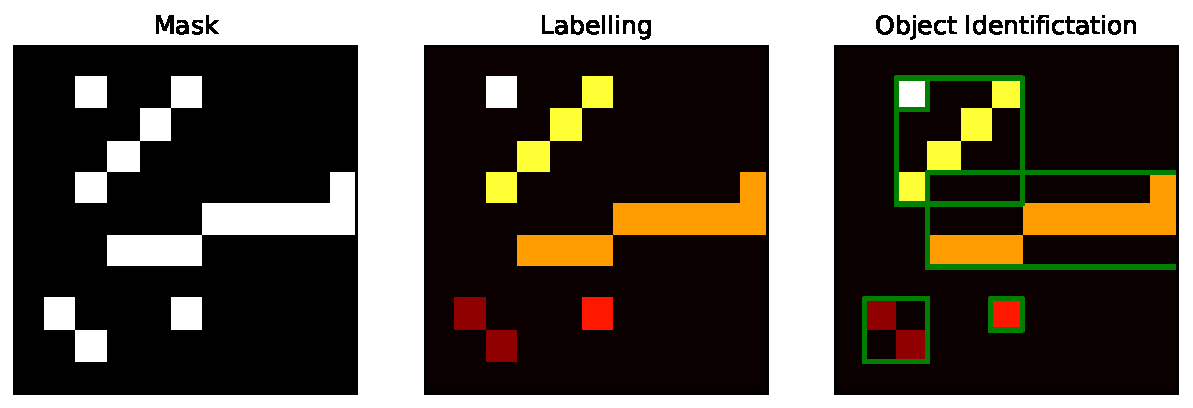
\includegraphics[width=\textwidth]{images/TrackObs_Objects}
  \caption{Identification of individual connected objects from a cosmic ray mask. The boolean mask (left panel) is used to calculate an integer array for all 8-connected pixels, which are labeled with a unique integer per object (middle panel). Objects are then identified by their labels as rectangular image sections around all pixels with a common label (green boxes in right panel).}
  \label{fig:TrackObs_Objects}
\end{figure}

First, individual objects are identified from the mask. This process is shown in Figure \ref{fig:TrackObs_Objects}. From the boolean mask, a labelling algorithm from the \texttt{scipy} Python distribution is used to assign the same integer value to all neighbouring pixels set to True -- in this case, if they are horizontally, vertically or diagonally adjacent. The labelled array is then used by a \texttt{scipy} object finding algorithm to identify the bounding boxes of all pixels of the same label.

Each TrackObs then contains an array whose rows represent information on one of the objects identified in the above steps. For each track, it lists:
\begin{itemize}
  \item The AL and AC lengths of the bounding box
  \item The location of the track, encoded as the lowest AL and AC value in its bounding box
  \item The sub-image of the track from the signal array, encoded in ADU. Note that this only includes those pixels inside the bounding box with the corresponding label - in the right panel of Fig. \ref{fig:TrackObs_Objects}, the image of the $4 \times 4$ diagonal track in the upper left does not include the single pixel track in its bounding box, which has a different label.
  \item The sum of signal values of the track in electrons, corresponding to the total measured ionizing energy.
  \item The uncertainty of the total ionizing energy, being the square root of the sum of the squares of the individual pixel uncertainties.
\end{itemize}

Each of the following algorithms produces such TrackObs objects, which are saved intermediately as FITS files.




\subsubsection{SM-SIF: Laplacian Edge Detection}
\begin{figure}
  \centering
  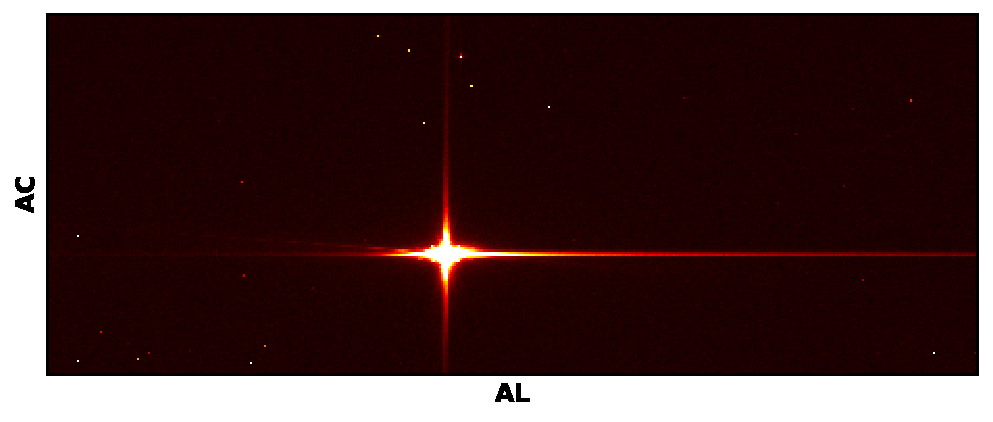
\includegraphics{images/SM_full_image}
  \caption{An example of a SM-SIF source image. Axis orientation is the standard Gaia convention, with the serial register to the right and readout to the upper right corner. The aspect ratio has not been corrected for pixel geometry and binning.}
  \label{fig:SM_full}
\end{figure}

Figure \ref{fig:SM_full} demonstrates a typical image in the SM-SIF dataset. The image contains a bright star object with a PSF that contains long diffraction spikes and a saturated core. Smaller stars and what appear to be cosmic ray tracks can be detected by bare eye.

To automate the detection of cosmic ray tracks in these images, they must be successfully separated from the imaged astronomical objects. Such algorithms, usually used to remove unwanted cosmic rays, have been developed for earlier ground- and space-based observatories and can be used in to our advantage. For this dataset, we decided to utilize the \textsc{L.A. Cosmic} algorithm described in \cite{Dokkum_cosmics}. Briefly summarized, this algorithm utilizes a variation of Laplacian edge detection to discriminate cosmic ray tracks from stars by their sharp edges, which separates them from the smoother PSFs of stars.

In more detail, the algorithm first convolves a subsampled version of the original image with a derivative filter, which assigns high values to sharp edges. The resulting image is compared with a noise image, calculated by a $5 \times 5$ median filter of the image and including the CCD readout noise. Pixels with a signal-to-noise-ratio above a high threshold are then selected as first candidates for noise pixels, after which a lower threshold is applied to neighbouring pixels. The identified pixels are then masked and the original image is cleaned, replacing the cosmic ray pixels with the median or mean of the surrounding, unmasked pixels. This procedure, starting from the convolution, is applied iteratively until either no more pixels are identified or the maximum number of iterations has been reached.

This analysis utilizes a Python implementation of the \textsc{L.A. Cosmic} algorithm called \textsc{Astro-SCRAPPY} \cite{astroscrappy} for cosmic ray identification.

First attempts at simply applying \textsc{Astro-SCRAPPY} to images like the one in Fig. \ref{fig:SM_full} revealed that the bright stars in most of the SM-SIF images were still falsely detected as cosmics. The reason for this is their saturation of the detector -- see especially the middle panel of Figure \ref{fig:SM_starmask}. The bright star, as it saturates the detector, causes a strong blooming effect, saturating even the pixels read in after those exposed to the bright stars (the image read out direction is to the top). As the panel shows, the resulting pattern has a very sharp gradient, which is picked up by the Laplacian filter and mis-identified as a cosmic.

\begin{figure}
  \centering
  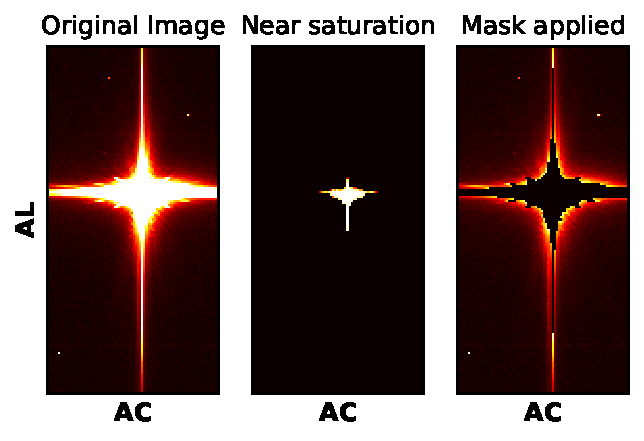
\includegraphics{images/SM_starmask}
  \caption{Bright stars in SM-SIF and their masking. \textit{Left:} The appearance of the bright star from Fig. \ref{fig:SM_full}. \textit{Middle:} The left panel after applying a high threshold. The bright pixels are fully saturated and show a sharp charge transfer pattern. \textit{Right:} The left panel after applying bright star filtering - the core and a large part of the diffraction spikes are masked.}
  \label{fig:SM_starmask}
\end{figure}

To eliminate these bright star cores and mask their extended field, in which cosmics will disappear under the poisson noise of the star, we apply a simple algorithm before extracting cosmics. Its steps are:
\begin{enumerate}
  \item Object finding: Construct a mask set to 1 for every pixel above a low threshold and apply object labelling to this mask. This step essentially catches all stars and cosmics.
  \item Saturated object identification: Of all objects, select only those that contain at least one pixel at a value of 65535 ADU, the maximum of a 16-bit integer. 
  \item Masking: Add all the objects identified in the previous steps to a mask (set to 1 for invalid pixels). This mask can be forwarded to \textsc{Astro-SCRAPPY}, which supports masked regions and does not use them for cosmic identification.
\end{enumerate}

The results of this algorithm can be seen in the right panel of Fig. \ref{fig:SM_starmask}, where all pixels belonging to the bright star are set to zero. There still remain some parts of the bright star's PSF - these, however, are very close to the bias level and decay smoothly, thus causing no issues.

Using the bright star removal, we then constructed the following algorithm to extract cosmics from SM-SIF observations:
\begin{enumerate}
  \item Read in the image and construct the bright star mask.
  \item Subtract the AL-dependent bias and apply the gain-scale, as \textsc{L.A. Cosmic} requires an image in units of electrons to calculate the Poisson noise.
  \item Apply \textsc{L.A. Cosmic}, which returns the cosmic ray mask and a cleaned image. The values of the cleaned image are calculated by taking the mean of the surrounding, non masked pixels in a $5 \times 5$ pixel area, i.e. for a pixel located at $\left(AL,AC\right)$, the cleaned value is
    \begin{equation*}
      \mathrm{Clean}\left(AL,AC\right) = \left( \sum\limits^\mathrm{mask=False}_{\substack{AL-2 \leq i \geq AL+2 \\ AC-2 \leq j \geq AC+2}} \mathrm{Source}\left( i, j \right) \right) \bigg/ \left( \sum\limits^\mathrm{mask=False}_{\substack{AL-2 \leq i \geq AL+2 \\ AC-2 \leq j \geq AC+2}} 1\right)
    \end{equation*}
  \item Calculate the signal array as $~\mathrm{Signal}\left(AL, AC\right)= \mathrm{Source}\left(AL, AC\right) - \mathrm{Clean}\left(AL, AC\right)$
  \item Calculate the uncertainty array as the square root of the variance of the signal array, calculated as
    \begin{equation*}
      Var\left(AL,AC\right) = \mathrm{Source}\left(AL,AC\right) + \sigma_\mathrm{rn}^2 + \sum\limits^\mathrm{mask=False}_{\substack{AL-2 \leq i \geq AL+2 \\ AC-2 \leq j \geq AC+2}} \frac{\mathrm{Source}\left(i,j\right) + \sigma_\mathrm{rn}^2}{N_\mathrm{mean}\left(AL,AC\right)},
    \end{equation*}
    with $\sigma_\mathrm{rn}^2$ denoting the pixel readnoise, and $N_\mathrm{mean}\left(AL,AC\right)$ denoting the number of pixels used to calculate the mean for cleaning this pixel. As one can see from the equation, the noise of the source image has been assumed to be Poissonian noise and readnoise.
  \item Extract tracks from the mask, signal and uncertainty images and save them as a TrackObs, as described above.
    
\end{enumerate}

\subsubsection{BAM-OBS: Boxcar filtering / Stacking}
\begin{figure}
  \centering
  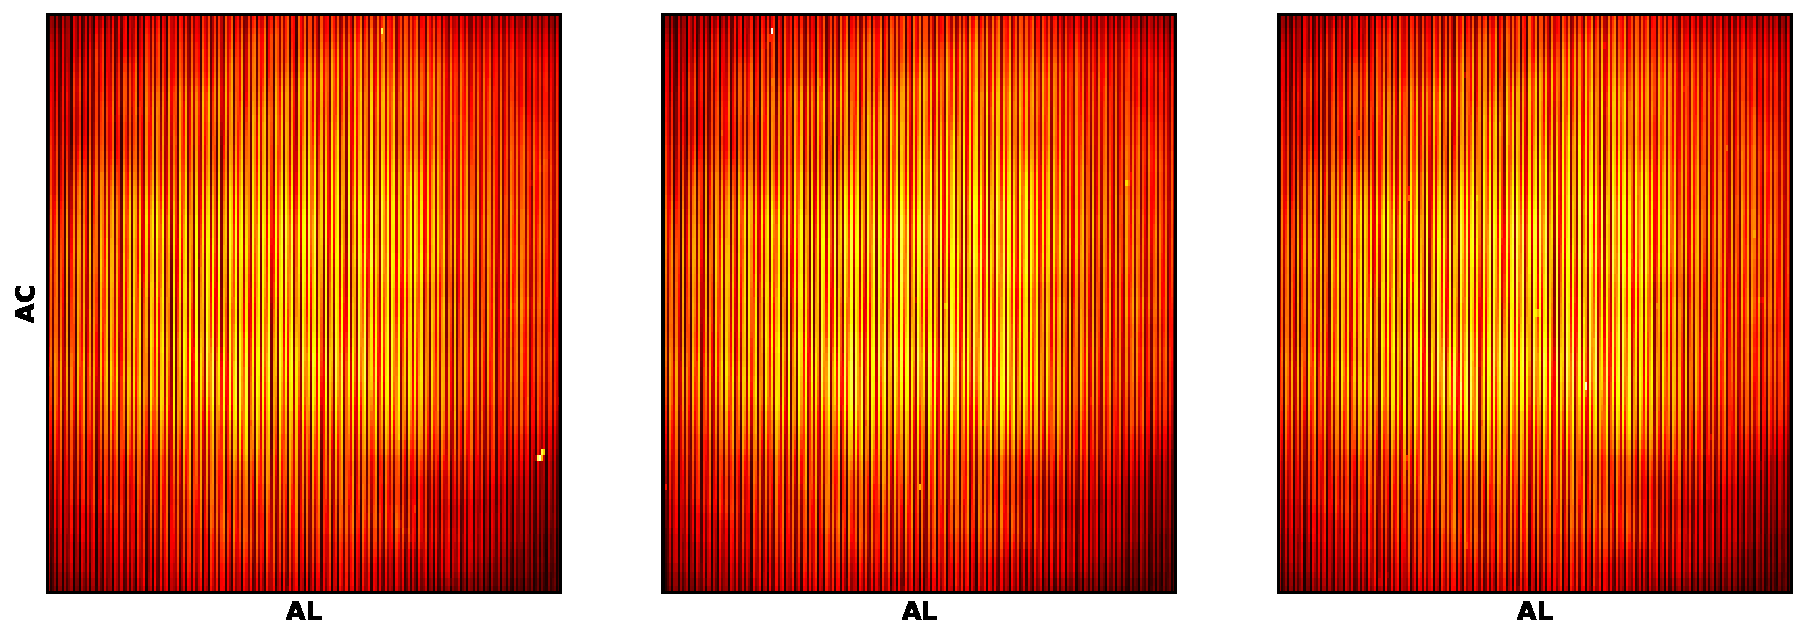
\includegraphics[width=\textwidth]{images/BAM-OBS_patterns}
  \caption{A series of three BamObservations from FOV 1. The dimensions have been rescaled to the physical dimension of the CCD -- each image pixel represents a $10 \times 120\, \mu m$ (AL $\times$ AC) sample. Individual pixels that deviate from the patterns can be recognized as cosmic ray tracks.}
  \label{fig:BAM_patterns}
\end{figure}

Figure \ref{fig:BAM_patterns} shows a series of observations from FOV 1 of the BAM. The three images were recorded in series (left to right) with an exposure time of about 23 seconds each. It is visibly apparent that the BAM patterns do not significantly between single observations, yet all three images contain pixels deviating from the pattern that only exist in one given image. These spurious pixels are a clear sign of cosmic rays.

\begin{figure}
  \centering
  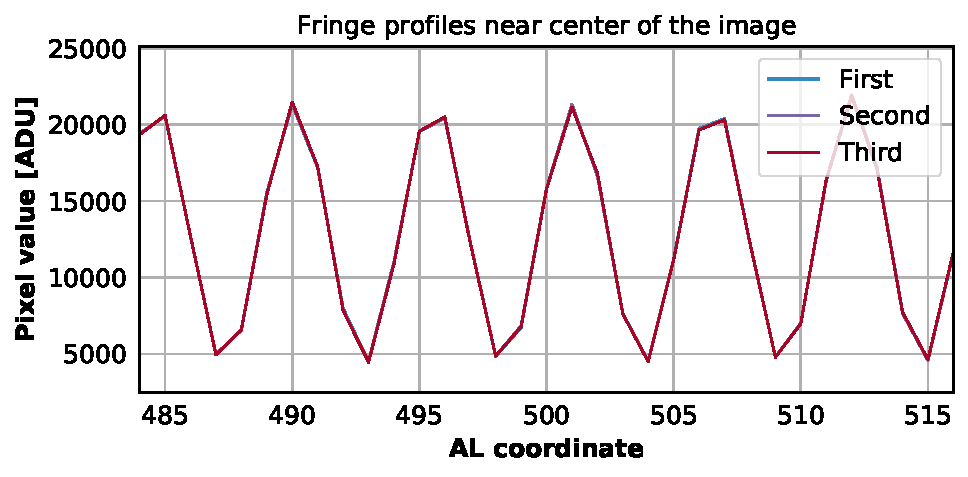
\includegraphics{images/BAM-OBS_fringes}
  \caption{The ADU values of the three patterns in Fig. \ref{fig:BAM_patterns} plotted along the center of the images in AC across a narrow AL region in the center. The interference pattern is very sharp, with a period of about 5 pixels in AL. The fringes of all three images overlap very closely.}
  \label{fig:BAM_fringes}
\end{figure}

Figure \ref{fig:BAM_patterns} further demonstrates that the interference pattern does not vary aside from Poissonian noise between the three images. It also shows why a simple application of the \textsc{L.A. Cosmic} algorithm to this dataset will immediately fail: The interference patterns themselves are very sharp, with a peak-to-trough distance of about 2 to 3 pixels. The algorithm is totally blinded by the pattern and can not separate it from the cosmics.

For our track extraction algorithm, we exploited the fact that the interference pattern is relatively static. In astronomy, multiple exposures of the same object (assuming constant luminosity) are used to reject the spurious high pixel values caused by cosmic rays -- a similar algorithm is used to reject cosmics in BamObservations when analyzing the pattern. In our case, we can simply do the reverse, and accept pixels that vary significantly stronger than the inherent counting and readout noise as the tracks of cosmic rays.

The concrete algorithm assumes as an input a time-ordered series of BamObservations from a single FOV, and operates on a range of observations, which we refer to as a BoxCar. To create a good estimate of the pattern across a period of time where it does not vary, we chose to use a total of 7 images at once - a central image for cosmic ray extraction and the three images recorded immediately after and before. The extraction algorithm works as follows.

\begin{enumerate}
  \item Construct the BoxCar: Read the first 7 BamObservations -- applying the electron conversion gain -- into a three dimensional array with the indices $t$, $AL$ and $AC$ - with $t \in [1,\cdots,7]$ ($t = 3$ being the central observation), and $AL$ and $AC$ denoting the image dimensions.
  \item Sigma-clipping: Compute the median and standard deviation across time and mark all the pixels whose difference to the median exceeds a chosen threshold - these are likely cosmics, and will not be used to calculate the pattern.
  \item Calculate a two-dimensional image array of the pattern, by taking the mean across time without using the sigma-clipped pixels, e.g.
\begin{equation*}
  \mathrm{Pattern}\left( AL,AC \right) = \left( \sum\limits_{t~\mathrm{not~clipped}} \mathrm{BoxCar}\left( t, AL, AC \right) \right) \bigg/ \left( \sum\limits_{t~\mathrm{not~clipped}} 1\right).
\end{equation*}
  \item Calculate the signal array by subtracting the Pattern from the central array in the BoxCar, e.g.
\begin{equation*}
  \mathrm{Signal}\left( AL,AC \right) = \mathrm{BoxCar}\left(t=3,AL,AC \right) - \mathrm{Pattern}\left( AL,AC \right).
\end{equation*}
  \item Calculate the uncertainty array as the square root of the variance of the signal array, calculated as
    \begin{equation*}
      Var\left(AL,AC\right) = \mathrm{BoxCar}\left(t=3,AL,AC\right) + \sigma_\mathrm{rn}^2 + \sum\limits_{t~\mathrm{not~clipped}} \frac{\mathrm{Boxcar}\left(t,AL,AC\right) + \sigma_\mathrm{rn}^2}{N_\mathrm{mean}\left(AL,AC\right)},
    \end{equation*}
  with $\sigma_\mathrm{rn}^2$ denoting the pixel readnoise, and $N_\mathrm{mean}\left(AL,AC\right)$ denoting the number of pixels in the BoxCar that have not been rejected by sigma clipping at this $\left(AL,AC  \right)$ pair. As one can see from the equation, the noise of the BamObservations has been assumed to be Poissonian noise and readnoise.
  \item Create the cosmic mask: Divide the signal array by the uncertainty array and create the boolean mask array, set to true where the signal/uncertainty ratio is greater than a threshold $f$. Due to the strong photon background, some cosmic pixels are missed in this step. We attempt to mitigate this by investigating all the pixels that neighbour the previously masked pixels, found via binary dilation, and applying for them a signal/uncertainty threshold of $r_\mathrm{Neighbour}*f$, adding the pixels that satisfy this condition to the mask as well.
  \item Apply a track connection algorithm: Even after the previous step, visually apparent long cosmic ray tracks still remain separated - refer to the left panel of Figure \ref{fig:BAM_connection} for an illustration. Tracks that are oriented in the AL direction see a strongly variable photon background, seen as fluctuations in the uncertainty array. These pixels are less likely to be detected by the thresholding of before. Especially towards the center of the image, where the pattern amplitude is very high, this leads to a single, long cosmic being detected as multiple short cosmics in the troughs of the interference pattern, which eventually leads to an overestimation of the cosmic ray rate.

    In an attempt to correct for this track separation, we implemented a track connection algorithm: We first apply to the mask an 8-connected binary dilation followed by a 4-connected binary erosion (this is a variant on binary closing, which uses the same structuring elements for the dilation and erosion instead), illustrated in the middle and right panels of Fig. \ref{fig:BAM_connection}. As the Figure shows, this marks several pixels of interest that may connect the separated objects.

    We then examine each of the newly merged tracks, which are identified by the standard labelling algorithm. For each of the tracks, we first calculate the mean of the previously identified signal pixels of this track, $m_\mathrm{Object}$. Assuming that a cosmic ray creating a long track should have a constant energy deposition per path length, we examine each of the candidate pixels (at the location $\left(AL,AC\right)$), checking for the condition
    \begin{equation*}
      \lvert Signal\left( AL,AC \right) - m_\mathrm{Object}\rvert > cfac * \sqrt{Var\left( AL,AC \right)},
    \end{equation*}
    with $cfac$ being an algorithm parameter. The above equation checks whether the signal value of the candidate pixel is sufficiently close to the value of the other pixels in this object. If a pixel satisfies the condition, it is added to the pixel mask. 
  \item Extract tracks from the mask, signal and uncertainty images and save them as a TrackObs, as in SM-SIF and described above.
  \item Update BoxCar: Read in the next BamObservation and replace the oldest pattern in the BoxCar with it -- the BoxCar is utilized as a FIFO, in this case. We then update the central pixel index and repeat starting step 2 until all BamObservations have been processed.
\end{enumerate}

\begin{figure}
  \centering
  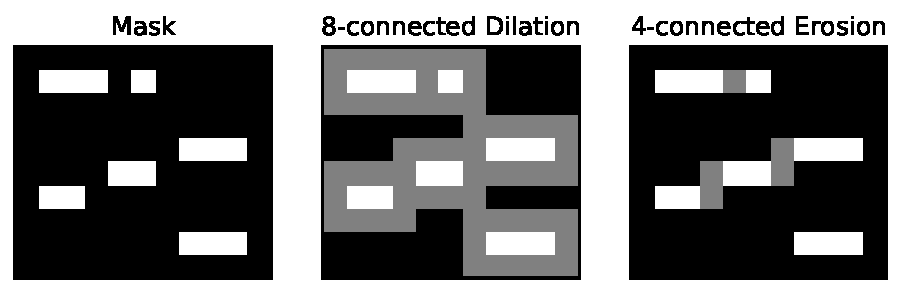
\includegraphics{images/BAM-OBS_connection}
  \caption{Illustration of the track connection algorithm used for this dataset. \textit{Left:} An example of a cosmic ray mask where ray tracks oriented in the AL direction have not been fully identified. \textit{Middle:} Application of 8-connected binary dilation to the mask - the added pixels are shown in gray. \textit{Right:} Additional application of 4-connected binary erosion, shown in the gray pixels, which are examined by the connection algorithm.}
  \label{fig:BAM_connection}
\end{figure}

\subsubsection{BAM-SIF: Thresholding}
\begin{figure}
  \centering
  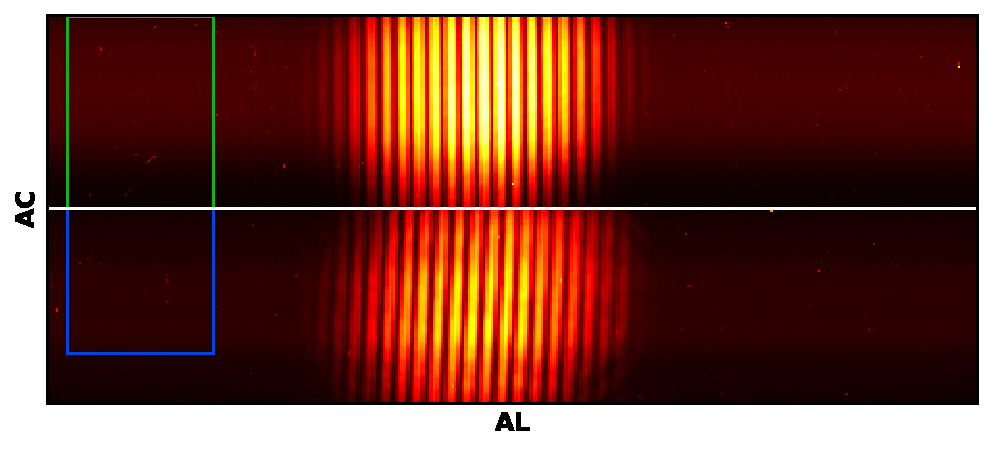
\includegraphics{images/BAM-SIF_full_image}
  \caption{An example of a BAM-SIF source image, which has been rescaled to the physical CCD dimensions. The top half of the image shows the AC region of FOV 2, the bottom half that of FOV 1. The off-pattern regions in green and blue boxes are used for cosmic extraction.}
  \label{fig:BAM-SIF_full}
\end{figure}

Figure \ref{fig:BAM-SIF_full} depicts an example for a BAM-SIF image used in this extraction. These images both contain the interference pattern in the BAM-OBS images, as well as off-pattern regions showing the TDI footprint of the pattern, which is only AC-dependent. These images are much less frequently sampled than the BAM-OBS images -- usually a handful of images twice per week -- which is why they are not very useful for the purpose of particle monitors. However, the off-pattern regions offer a good opportunity to extract cosmics from the BAM chip with a much lower and simpler background than that of BAM-OBS, allowing us to examine the effect the pattern has on the above extraction.

As this dataset is very attractive for cosmic ray extraction, it has been used before for cosmic ray studies, see \cite{GAIA-DE-TN-ESAC-RKO-033}. This algorithm builds on the previous extraction, merging it into the TrackObs-based files approach utilized here.

For the extraction of cosmics, we utilize the two regions outlined in blue and green boxes in Fig. \ref{fig:BAM-SIF_full}. A smaller region in AC has been selected for the FOV 1 region - the ignored region has shown a high stray light contamination, which causes mis-identifications.

The extraction algorithm for this dataset is then (for each region seperately):
\begin{enumerate}
  \item Read in the image and apply the gain scale.
  \item Determine the AC-dependent TDI background: Take the 99 columns with the highest AL value (to the left in Fig. \ref{fig:BAM-SIF_full}) and remove the outliers -- for each column within, discard the highest and lowest 25\,\% of pixel values to remove cosmics. Then, calculate the mean and standard deviation of the remaining image pixels for each line. The output are two one-dimensional arrays of the AC-dependent TDI background and its standard deviation.

    The removal of the TDI background is demonstrated in Figure \ref{fig:BAM-SIF_background}
  \item Calculate the signal and variance arrays as
    \begin{equation*}
      Signal\left( AL,AC \right) = Source\left( AL,AC \right) - Background\left(AC \right)
    \end{equation*}
    and
    \begin{equation*}
      Var\left( AL,AC \right) = Source\left( AL,AC \right) + \sigma_\mathrm{rn} + \sigma_\mathrm{Background},
    \end{equation*}
    with $\sigma_\mathrm{rn}$ being the readnoise and once again assuming Poisson noise in the source array. The uncertainty array is then the square root of the variance array.
  \item Construct the mask array in exactly the same way as for BAM-OBS, including the track connection. While this should not be necessary here, we want to have as similar as possible algorithms for BAM-OBS and BAM-SIF, to see the effect of the pattern.
  \item Extract tracks from the mask, signal and uncertainty images and save them as a TrackObs, as in the algorithms above.
\end{enumerate}

\begin{figure}
  \centering
  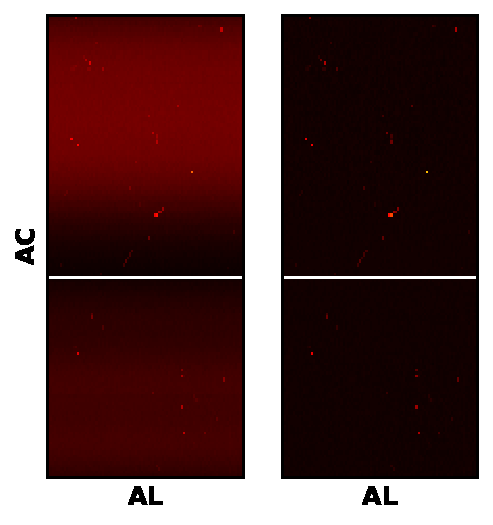
\includegraphics{images/BAM-SIF_background}
  \caption{\textit{Left:} The two extraction regions from Fig. \ref{fig:BAM-SIF_full}. \textit{Right:} The same image with the TDI backround removed, leaving only cosmic ray tracks.}
  \label{fig:BAM-SIF_background}
\end{figure}

All steps until the calculation of the signal are the same as in \cite{GAIA-DE-TN-ESAC-RKO-033}, which only returned the signal images.

\subsection{Post-Processing}

\subsubsection{Observed Flux}

\subsubsection{Track Geometries}

\subsubsection{Flagging Special Tracks}

i.e. those at the edge of the readout windows. Maybe also the removal of tracks at obviously too low energies?


\section{Data Model}
\label{sec:datamodel}

{\textbf DEPRECATED}

This data model is composed of entities {\it ParticleEvent} which are described in full detail in the following subsection.

\subsection{Data Model Description}

\textbf{Entity Name}:  \textit{ParticleEvent}
\newline
\newline
\textbf{Entity Description}:  A cosmic ray (prompt particle event) detection from any of the analyzed Gaia CCDs 
\newline
\newline
\textbf{Entity Attributes}:
\newline
\begin{table}[!h]
\centering
\resizebox{\textwidth}{!}{\begin{tabular}{|l|l|l|l|}
\hline
{\textit{\textbf{Name}}} & {\textit{\textbf{Description}}} & {\textit{\textbf{Unit}}} & {\textit{\textbf{Type}}} \\ \hline
TRACK\_START\_POS\_AL & The start position of the event in the AL direction & pixel & Short \\ \hline
TRACK\_START\_POS\_AC & The start position of the event in the AC direction & pixel & Short \\ \hline
TRACK\_LEN\_AL & Event track length in AL & pixel & Short \\ \hline
TRACK\_LEN\_AC & Event track length in AC & pixel & Short \\ \hline
TRACK\_EN & Event track total energy  & electrons & Integer \\ \hline
TRACK\_EN\_ERR & Uncertainty in the event track total energy  & electrons & Integer \\ \hline
TRACK\_TRUNCATED & Is the event truncated by start/end of CCD physical area & NA & Boolean \\ \hline
EST\_PART\_LEN & Estimated incident particle track length (if applicable) & $\mu$m & Float \\ \hline
EST\_PART\_LEN\_ERR & Uncertainty in the estimated incident particle track length (if applicable) & $\mu$m & Float \\ \hline
EST\_PART\_THETA & Estimated incident particle impact angle (if applicable) & deg & Float \\ \hline
EST\_PART\_THETA\_ERR & Uncertainty in the estimated incident particle impact angle (if applicable) & deg & Float \\ \hline
\end{tabular}}
\caption{Event detection data model version \dmVersion}
\end{table}

% Questions:
% - users may also be interested in track lengths in SI units, e.g. micrometers
% - will we provide extra info on the binning for individual data products, or give the pixel coordinates of the samples (which implicitly include the binning)?
% - are angles already with respect to some external reference e.g. the sun? We may need two angles for a full description (angle of focal plane wrt sun AND angle of the cosmic on the focal plane)
% the focal plane to sun angle will be interesting in any case during solar flares, as this should lead to an additional modulation in flux
% should TRACK_EN be in keV? the conversion is a constant (pair production energy in SI)
% I suppose EST_PART_EN would be for protons?

\subsection{Event Track Reconstruction}

We should describe here (TBD if needed) a simple way to reconstruct the window for a given detection from the provided data.

\section{Persistence Considerations}
\label{sec:persist}
\subsection{Persistence Method(s)}

We should describe here the proposed persistence methods (different alternatives file system based or database), with pros and cons.

\subsection{Size Estimations}

Catalog size estimation is a function of :
\begin{enumerate}
\item The technology used for the generation of this catalog. 
\item The persistence format or system used for storage.
\end{enumerate}

Detection algorithms have been developed and written in Python and the default persistence method adopted is TBD. This results in the following estimations.
\newline
\newline
\textbf{Note:} the following estimations are applicable to catalog version : \dmVersion  
\newline
\newline

Assuming an average event rate (in the absence of solar activity) of : 5 events/s , the average volume of the catalog per spacecraft revolution is : x bytes. Since Gaia performs 4 full revs on it's spin axis every 24 hrs, the average catalog volume per 24 hrs is : y bytes. This needs then to be multiplied by the total nb of mission days covered by the corresponding version of the catalog. 

\subsection{Long Term Preservation}

\section{Quality Control Metrics}
\label{sec:metrics}
Every run of the batch processing cosmic ray detection algorithms shall generate a new version of the catalog. The corresponding version of the catalog will be quality control checked prior to it's official release.

\subsection{Internal Consistency Checks}

\subsection{External Consistency Checks}

\section{Catalog Release Mechanism}
\label{sec:release}
\subsection{Catalog Version Generation}

The proposed catalog versioning scheme is as follows: \newline\newline  \textit{vN.m} \newline\newline where 

\begin{itemize}
\item \textit{N} is a \textit{major} version of the catalog, only updated due to schema updates (i.e, new attributes added or modifications to existing attributes).
\item \textit{m} is a \textit{minor} version of the catalog updated when a new batch processing is performed \textbf{after} algorithmic or software updates. 
\item executions of a new batch processing with no software or algorithm updates but over an increased mission time range result in the increment of the \textit{minor} version of the catalog.

\end{itemize}

Every new version of the catalog (major or minor) will be quality control checked prior to it's official release, according to the criteria described in section~\ref{sec:metrics}.

\subsection{Release Mechanism and Notification to Users}

This is TBD.


\begin{thebibliography}{9}
\bibitem{GAIA-CA-SP-ARI-BAS-003} U. Bastian \emph{Reference Systems, Conventions And Notations for Gaia}.
\bibitem{GAIA-DE-TN-ESAC-RKO-033} R. Kohley \emph{Cosmic rays on BAM CCDs data delivery note}.
\bibitem{Dokkum_cosmics} P. G. van Dokkum \emph{Cosmic-Ray Rejection by Laplacian Edge Detection}.
\bibitem{astroscrappy} C. McCully \emph{Astro-SCRAPPY: The Speedy Cosmic Ray Annihilation Package in Python}, \url{https://github.com/astropy/astroscrappy}.


\end{thebibliography}

\end{document}
